\documentclass[a4paper,fleqn]{cas-dc}

\usepackage[numbers]{natbib}
\usepackage{amsmath, amsfonts, amssymb}
\usepackage{algorithm, algpseudocode}
\usepackage{graphicx}
\usepackage{adjustbox}
\usepackage{xcolor}
\usepackage{booktabs, tabularx, multirow}
\usepackage{enumitem}
\usepackage{ragged2e}
\setlist{nosep}
\newcommand*\D{\mathop{}\!\mathrm{d}}
% Your custom definitions or commands here
% For colouring in the results tables
\definecolor{darkblue}{RGB}{0,0,139}
% Define new column types for the 4th and 5th columns
\newcolumntype{B}{>{\bfseries\textcolor{darkblue}}c}
\newcolumntype{C}{>{\bfseries\textcolor{darkblue}}c}


\begin{document}

% Title
\shorttitle{Higher-Order Greeks Hedging of American Options with DRL}
\shortauthors{Tsoskounoglou et~al.}

\title[mode=title]{Higher-Order Greeks Hedging of American Options \newline with Deep Reinforcement Learning}

% Author(s)
\author[1]{Alexander Tsoskounoglou}[]
\ead{alexander.tsoskounoglou@gmail.com}

\author[1,2]{Sven Karbach}[]
\ead{sven@karbach.org}
\fnmark[1]

\author[1,2]{Drona Kandhai}[]
\ead{b.d.kandhai@uva.nl}
\fnmark[1]

\author[3]{Michel Vellekoop}[]
\ead{m.h.vellekoop@uva.nl}

\fntext[fn1]{The authors acknowledge support from the AI4FinTech initiative at the University of Amsterdam.}
% Corresponding author
%\cormark[1]
%\cortext[cor1]{Corresponding author}


\affiliation[1]{%
  organization={Informatics Institute, University of Amsterdam},
  addressline={LAB42, Science Park 900},
  city={Amsterdam},
  postcode={1098 XH},
  country={The Netherlands}
}

\affiliation[2]{%
  organization={Korteweg-de Vries Institute for Mathematics, University of Amsterdam},
  addressline={Science Park 105–107},
  city={Amsterdam},
  postcode={1098 XG},
  country={The Netherlands}
}

\affiliation[3]{%
  organization={Faculty of Economics and Business, University of Amsterdam, Section Quantitative Economics},
  addressline={Roetersstraat 11},
  city={Amsterdam},
  postcode={1001 NJ},
  country={The Netherlands}
}


% Abstract
\begin{abstract}
This paper studies a hedging framework for American options that addresses the practical challenges posed by early exercise, transaction costs, and higher-order risk exposure. We combine PDE-based option pricing under the Heston stochastic volatility model using the modified Craig–Sneyd scheme with a distributional deep reinforcement learning (DRL) approach to learn adaptive hedging strategies. Unlike traditional methods, our DRL agent optimizes directly for tail-risk objectives, including Value-at-Risk and Conditional Value-at-Risk, while accounting for transaction cost constraints and limited re-balancing frequency. Through extensive numerical experiments, we demonstrate that the proposed DRL framework consistently outperforms Delta-Gamma and Delta-Vega hedging, particularly in high-cost regimes where complete higher-order neutrality is impractical. Specifically, our method reduces VaR by approximately 17.1\% compared to Delta-Gamma strategies and up to 39.4\% relative to Delta-Vega approaches. Moreover, the learned strategies remain robust under misspecification of key Heston parameters such as the asset-volatility correlation. The robustness results support the practical applicability of our approach, enabling effective higher-order risk management even in the presence of model uncertainty.
\end{abstract}


% Highlights
%\begin{highlights}
%\item Introduced a DRL framework for higher-order American option hedging under the Heston model.
%\item Simulated stock trajectories using the Quadratic-Exponential scheme.
%\item Combined MCS PDE pricing and with D4PG-QR distributional reinforcement learning.
%\item Achieved superior tail-risk and cost performance vs. Delta-Gamma/Vega hedging.
%\item Incorporated transaction costs and early exercise in a realistic hedging setup.
%\item Demonstrated robustness to model misspecification in key Heston parameters.
%\end{highlights}

% Keywords
\begin{keywords}
Deep Reinforcement Learning \sep American Options \sep Heston Model \sep Transaction Costs \sep Hedging \sep PDE pricing
\end{keywords}

\maketitle

% ===============================================================
% ===============================================================
% ===============================================================


% =============================================================
% =============================================================
% =============================================================

\section{Introduction}
\label{Introduction}

Hedging American options presents substantial challenges due to early exercise features, transaction costs and frequent rebalancing requirements. These complexities further increase when looking at portfolios of American options or the sequential issuance of option liabilities. In volatile markets, managing higher-order Greeks, particularly Gamma and Vega, is essential for further reducing risk, as Delta hedging alone is insufficient. Traditional methods for pricing American options based on binomial trees~\cite{ccr} or finite difference methods~\cite{FDM_american} have proven effective under both constant and stochastic volatility models, including the Heston framework~\cite{hestonModel}. However, when directly applied to hedging, these approaches typically assume frictionless markets and continuous trading. In practice, this leads to unrealistic strategies characterized by excessive rebalancing and elevated transaction costs, while still leaving significant tail-risk exposures unaddressed. Consequently, practical hedging demands cost-aware adaptive methods that dynamically balance risk exposure and trading efficiency.

Recent advancements in \emph{Deep Reinforcement Learning} (DRL) have shown to address the complexities of hedging under realistic market conditions effectively~\cite{DH_R, DH_2}. Unlike classical methods, DRL-based strategies explicitly incorporate market frictions during policy training, enabling adaptive hedging that balances risk minimization, in particular the tail risk measured via Value-at-Risk (VaR) or Conditional VaR (CVaR), against transaction costs. However, most existing DRL literature focuses on European-style options~\cite{DH_01, DH_1, DH_3}, where early exercise is not permitted, and the associated option evaluation is comparatively simpler. Robust DRL frameworks specifically tailored for American-style options, particularly put options, which are frequently exercised early, remain scarce~\cite{DH_A}. Moreover, existing studies often concentrate solely on Delta hedging or rely on simplified asset dynamics. As a result, the accurate and cost-aware management of higher-order Greeks under realistic conditions, including transaction costs and stochastic volatility, has not been comprehensively addressed in the literature~\cite{buhler2019deep, zheng2023option, murray2022deep, giurca2021delta}. 

\subsection{Main Contributions}
To address these gaps, this paper proposes an advanced DRL framework specifically designed for dynamic hedging of American options under realistic market conditions, including stochastic volatility and transaction costs. The principal contributions of this paper are:

\begin{itemize}[noitemsep, left=4pt]
    \item \textbf{Distributional DRL Algorithm:} We extend the D4PG-QR algorithm \cite{DH_1} to optimize higher-order Greeks hedging policies for American options explicitly with respect to tail-risk metrics such as VaR and CVaR, and transaction costs, offering improved risk management over standard mean-based DRL approaches.

    \item \textbf{Detailed Benchmarking and Robustness Analysis:} The proposed DRL policies are rigorously benchmarked against classical Delta, Delta-Gamma, and Delta-Vega strategies across varying transaction cost regimes and models. Moreover, we demonstrate the robustness of the learned hedging strategy to model parameter misspecifications in the Heston stochastic volatility model.
\end{itemize}

\vspace{0.5em}
\noindent In addition, the paper makes two computational contributions:

\begin{itemize}[noitemsep, left=4pt]
    \item \textbf{Accurate Heston Simulation under QE Scheme:} In contrast to prior work relying on simplified volatility dynamics, we employ the \emph{robust Quadratic-Exponential} scheme \cite{heston_sim} to simulate asset paths in the Heston stochastic volatility model. This approach preserves the essential distributional characteristics of the underlying Cox--Ingersoll--Ross (CIR) process, ensuring that volatility paths remain strictly positive and follow realistic trajectories. This is crucial for accurate use of calibrated Heston parameters, as na\"{i}ve schemes like Euler-Maruyama introduce biases which results in inconsistencies between calibration and simulations.
    \item \textbf{Integration of Advanced PDE Pricing Methods:} We incorporate the \emph{Modified Craig--Sneyd Alternating Direction Implicit} method \cite{MCS_og} for efficient and accurate pricing of American options in the Heston framework. This method yields reliable Greek sensitivities required for effective higher-order hedging.
\end{itemize}

\vspace{0.5em}
\noindent In this paper, we conduct extensive numerical experiments and demonstrate that the proposed DRL framework significantly outperforms classical Greek-based hedging strategies, improving both risk reduction and cost efficiency, especially so in high transaction cost regimes. In particular, our DRL approach reduces VaR by approximately 17.1\% compared to Delta-Gamma hedging and up to 39.4\% relative to Delta-Vega hedging, showing the effectiveness of adaptive, risk-aware policy learning (see Table~\ref{table:gbmtable} and Table~\ref{table:hestontable} below).

\subsection{Structure of the Paper}
\label{sec:structure}

The remainder of this article is organized as follows. Section~\ref{sec:framework} formalize the hedging problem, details the stochastic models, option–pricing schemes, and the distributional DRL algorithm. Section~\ref{sec:experiments} presents the main empirical results obtained under a realistic market regime with positive interest rates and negative market price of vol-risk, benchmarking the learned strategy against Delta, Delta–Gamma, and Delta–Vega hedges. Complementary experiments carried out in a drift‑free setting are reported in Section~\ref{sec:experiments-with-zero-drift} to isolate the influence of early exercise incentives. Section~\ref{sec:robustness} then assesses the robustness of the policy to misspecification of Heston parameters. Finally, Section~\ref{sec:conclusion} summarizes the key findings, and Section~\ref{sec:FutureDirections} outlines avenues for future research.

% =============================================================
% =============================================================
% =============================================================
\section{Hedging Problem and DRL Framework}
\label{sec:framework}

The core objective addressed in this paper is the development of an optimal dynamic hedging strategy for a portfolio of American-style put options, with particular emphasis on managing higher-order risks, specifically Gamma and Vega. The hedging instruments to do so are the underlying asset, as well as additional American put options written on the same underlying asset. 

Focusing on the higher-order aspect of the portfolio, we employ a Deep Reinforcement Learning framework that directly optimizes the sequence of hedging decisions. The DRL agent learns the optimal dynamic policy throughout the option's life-cycle including the initial hedge position $\alpha_0$ at time zero. The market dynamics are simulated with a stochastic process of choice, using a set of parameters, which are assumed to remain constant during the hedging period. More precisely, the underlying asset price process $(S_t)_{t \geq 0}$ and its instantaneous variance process $(v_t)_{t \geq 0}$ are simulated under either a stochastic volatility model, in our case the Heston model, or the Geometric Brownian Motion (GBM) as a baseline. At each discrete re-balancing interval, the agent determines the optimal quantity of hedging instruments to minimize risk exposure measured by a risk metric such as Value-at-Risk over the full hedging horizon. Option prices and Greek sensitivities are computed at each time step based on the simulated market state $(S_t, v_t)$, in addition to the fixed set of initially calibrated model parameters.


\subsection{Modeling the Underlying (Physical Measure)}
\label{sec:ModelAssumptions}
In this study, we employ two primary models to simulate (underlying) asset price paths: the classical Black–Scholes (BS) model based on a GBM and the Heston stochastic volatility model. 

\paragraph{Black–Scholes Model}
Under the physical measure $\mathbb{P}$ the GBM dynamics are
\begin{align*}
\D S_t = S_t\,(r+\mu - q)\,\D t + S_t\,\sigma\,\D W_t, \quad t>0,
\end{align*}
where $\sigma$ is the constant volatility, $r$ is the risk‑free rate, $q$ is the continuous dividend yield, $\mu$ represents the excess mean rate of return on equity under~$\mathbb{P}$, and $(W_t)_{t\ge 0}$ is a standard Wiener process under $\mathbb{P}$.

\paragraph{Heston Model}
The Heston stochastic volatility model reads
\begin{align*}
\D S_t &= S_t\,(r+\mu - q)\,\D t + S_t\sqrt{v_t}\,\D W_t^{S}, \quad t>0,\\
\D v_t &= \kappa_{\mathbb{P}}\big(\theta_{\mathbb{P}} - v_t\big)\,\D t + \xi \sqrt{v_t}\,\D W_t^{v}, \quad t>0,
\end{align*}
where $(W_t^{S})_{t\geq 0}$ and $(W_t^{v})_{t\geq 0}$ are standard Wiener processes under $\mathbb{P}$ with correlation $\rho$, i.e., $\D\langle W^{S}, W^{v}\rangle_t=\rho\,\D t$. The parameters $\xi$, $\kappa_{\mathbb{P}}$, and $\theta_{\mathbb{P}}$ denote the vol‑of‑vol, the speed of mean reversion, and the long‑run mean of the variance process, respectively.


\paragraph{Simulation Methods.}
For the BS model we sample paths from its closed form solution. In contrast, Heston model paths are simulated using the robust Quadratic-Exponential (QE) scheme~\cite{heston_sim}, which is well-known for its numerical stability and its ability to preserve key distributional properties of the Heston model, including accurate moment matching of the CIR stochastic volatility process.

\subsection{American Option Pricing} 
The valuation of American put options in the BS model is done via the binomial tree approach~\cite{ccr} using a $200$-step tree and the valuation of American put options under the Heston model is performed using the modified Craig–Sneyd finite-difference scheme~\cite{MCS_og, hestonADI}. This choice is justified due to its numerical stability, efficiency, and the accurate computation of the options sensitivities (Greeks), which is a crucial property for our higher-order hedging set-up. The scheme numerically solves the following partial differential inequality subject to an early exercise condition:

\begin{multline*}
\frac{\partial U}{\partial t} 
+ \frac{1}{2} v S^2 \frac{\partial^2 U}{\partial S^2} 
+ \rho \xi S v \frac{\partial^2 U}{\partial S \partial v} 
+ \frac{1}{2} \xi^2 v \frac{\partial^2 U}{\partial v^2} \\
+ (r - q) S \frac{\partial U}{\partial S} 
+ \kappa_{\mathbb{Q}}(\theta_{\mathbb{Q}} - v) \frac{\partial U}{\partial v} 
- r U \leq 0,
\end{multline*}
and such that $U \geq (K - S)^+ $. In our implementation, a $50 \times 25$ grid in the stock and volatility dimensions provides a reasonable trade-off between computational cost and pricing accuracy, which allows us to simulate a high number of option prices required for the training and evaluating of the DRL agent %(see~\cite{tsoskounoglou2025msc} for more details). 


\subsection{DRL Framework for Hedging}

The hedging task is formulated as a \emph{Markov Decision Process} and is solved through a distributional deep-reinforcement learning algorithm. In particular, we define the state $s_t$, action $a_t$, and reward $R(s_t, a_t)$ at time $t$, which we use to manage risk exposure under market frictions, i.e. the exposure to the two Greeks Gamma and Vega under transaction costs. Delta hedging is assumed to be frictionless and $\Delta$ is absent from the state space $s_t$. In practice, the net delta of a call–put combination is typically small, as the call’s positive delta largely offsets the put’s negative delta.
\paragraph{State Space.} 
The state at time $t$ is defined by the vector,
\begin{align*}
    s_t = \{ S_t,\ \Gamma^{\text{Tot}},\ \mathcal{V}^{\text{Tot}}_t,\ \Gamma^{\text{Hedg}}_t,\ \mathcal{V}^{\text{Hedg}}_t \},
\end{align*}
where:
\begin{itemize}[noitemsep, left=10pt]
    \item $S_t$ is the current price of the underlying asset,
    \item $\Gamma^{\text{Tot}}_{t}$ and $\mathcal{V}^{\text{Tot}}_{t}$ denote the total aggregated Gamma and Vega exposure of the portfolio at time $t$, respectively. The total portfolio consists of the Delta portfolio, the liability portfolio, and the hedging portfolio,
    \item $\Gamma^{\text{Hedg}}_{t}$ and $\mathcal{V}^{\text{Hedg}}_{t}$ represent the Gamma and Vega of the available hedging option, which has 30 days to maturity and strike $K = S_t$ at time $t$.
\end{itemize}

Note that the instantaneous variance process $v_t$ does not appear explicitly in the state representation, but enters implicitly through the Gamma and Vega sensitivities.

\paragraph{Action Space.}
We model a continuous action space $\mathcal{A}:= [X_{\min}, X_{\max}]$. The action $a_t \in \mathcal A$ denotes the number of option shares to purchase at time $t$ for hedging purposes. These options are written on the same underlying asset as the rest of the portfolio, but can have different maturity from it. By dynamically adjusting the hedge position, the agent aims to reduce the portfolio's Gamma and Vega exposures, achieving either partial or full hedging. The bounds $X_{\min}$ and $X_{\max}$ correspond to hedging 0\% and 100\% of the Gamma or Vega risk. Specifically, $X_{\min}$ is set based on the lower of the Gamma or Vega exposure, while $X_{\max}$ reflects the higher of the two.


\paragraph{Reward Function.} 
The per-step reward is defined as:
\begin{align}
R(s_t, a_t) = \text{PnL}_{t \to t+\Delta t}^{\text{Tot}} - \text{TC}_t,
\end{align}
where $\text{PnL}_{t \to t+\Delta t}^{\text{Tot}}$ denotes the profit and loss of the total portfolio over the interval $[t, t+\Delta t]$, and $\text{TC}_t$ represents the transaction costs incurred at time $t$. The reward thus explicitly captures both portfolio profit/loss and trading costs. The DRL agent learns to optimize the cumulative reward over time, with a focus not only on expected return, but also on tail-risk management. To this end, we employ a distributional reinforcement learning approach based on quantile regression~\cite{DH_1, DH_01}, enabling direct optimization of tail-risk objectives such as VaR and CVaR and Mean-Std.

\paragraph{Policy and Discount Factor.}
The hedging policy $\pi(a\,|\,s)$ is a conditional distribution that assigns to every observed market state $s_t\in\mathcal S$ a feasible hedge adjustment $a_t\in\mathcal A$.  Given such policy, the agent generates a path which contains a set of states and decisions $\{(s_t,a_t)\}_{t=0}^{T-1}$ and stores a reward stream $R(s_t,a_t)$ defined previously.  For any coherent objective (risk) function $\mathcal{G}$, the optimisation problem becomes
\begin{equation*}
\pi^{*}
= \arg\max_{\pi}\;
\mathcal{G}\Bigl[\,
\textstyle\sum_{t=1}^{T}\gamma^{\,t}R(s_t,a_t)
\,\Bigr],
\qquad a_t\sim\pi(\cdot\mid s_{t-1}).
\end{equation*}
For example, under a VaR$_{95\%}$ criterion this becomes
$\mathcal{G}=\mathcal{F}^{-1}_{0.95}$.  
The discount factor $\gamma\in(0,1]$ controls how strongly rewards realised later in the hedge horizon influence the risk measure; we set $\gamma=1$, treating profit-and-loss at every step up to the $T\!=\!30$-day maturity with equal importance.

\paragraph{Objective Functions}
We evaluate risk using three commonly applied tail-sensitive metrics, each serving as a potential training and evaluation objective for the DRL agent. Let $\text{PnL}$ denote the cumulative profit and loss of the total portfolio. The objective functions are as follows:
\begin{align*}
    \text{Mean-Std} &= \mathbb{E}[\text{PnL}_t] - 1.645 \cdot \text{Std}[\text{PnL}_t] \\
    \text{VaR}_{95\%} &= \mathcal{F}^{-1}_{0.05}[\text{PnL}_t] \\
    \text{CVaR}_{95\%} &= \mathbb{E}[\text{PnL}_t \mid \text{PnL}_t \leq \text{VaR}_{95\%}]
\end{align*}
Here, Mean-Std penalizes variability around the expected return symmetrically by subtracting a multiple of the standard deviation. In a normal distribution a z score of -1.645 corresponds to the 95th quantile, and as shown in Figure ~\ref{fig:cvar_viz} in our case is very close to the 95th as well. VaR$_{95\%}$ targets the 95th percentile of the PnL distribution, identifying extreme losses with a fixed quantile cutoff. CVaR$_{95\%}$ measures the expected loss conditional on exceeding the VaR threshold, thus providing a deeper assessment of tail risk.

\subsection{Distributional Actor–Critic Algorithm}

We employ the D4PG-QR algorithm~\cite{DRL_3, DH_1}, which integrates continuous control with distributional reinforcement learning. By modeling the full return distribution via quantile regression, this approach enables direct optimization of VaR and CVaR, outperforming standard mean-based reinforcement learning methods.

\begin{itemize}[noitemsep, left=10pt]
    \item \textbf{Actor network}: outputs the continuous hedge adjustment $a_t$ given the current state $s_t$.
    \item \textbf{Critic network}: estimates the distribution of future returns using quantile regression, enabling explicit optimization of risk-sensitive objectives.
\end{itemize}

\paragraph{Training Procedure.} 
To create the simulated hedging environment, first, the underlying asset paths are generated (using either the Quadratic-Exponential scheme for the Heston model or the closed-form solution for the BS). Second, for each time step, PDE-based option prices and Greeks are computed for the option portfolios. Third, the DRL agent learns optimal hedging through the following iterative procedure: 

\begin{enumerate}[noitemsep, left=10pt]
    \item Transitions $(s_t, a_t, r_t)$ are collected and stored in a replay buffer.
    \item The critic network is updated off-policy by minimizing the distributional Bellman error via quantile regression.
    \item The actor network is updated using the policy gradient, guided by feedback from the distributional critic.
\end{enumerate}

\paragraph{Evaluation and Robustness Testing.} 
The trained DRL policy is evaluated out-of-sample on 8,000 episodes, which are simulated from the underlying models, to assess performance and generalization. Specifically, we test:
\begin{itemize}[noitemsep, left=10pt]
    \item Hedging performance relative to classical Delta, Delta-Gamma, and Delta-Vega strategies under various transaction cost regimes and objective functions.
    \item Robustness under misspecification of Heston model parameters: initial variance $v_0$, long-term variance $\theta_{\mathbb{P}}$, mean reversion speed $\kappa_{\mathbb{P}}$, vol-of-vol $\xi$ and correlation $\rho$.
\end{itemize}

\section{Experiments and Results}
\label{sec:experiments}

The framework required approximately 150,000 CPU hours for development and testing. Each Heston stochastic volatility scenario (e.g., 2\% transaction cost optimized with CVaR$_{95\%}$ objective) consumed around 1,440 CPU hours for simulation and training.

Transitioning from a constant volatility (BS) environment to the Heston model notably increased computational requirements, necessitating a doubling of training episodes from 32,000 to 65,000 and scaling parallelization from a single DRL agent to roughly 21 agents. This scaling addressed variability in hedging performance across training runs (see Figure~\ref{fig:cvar2}).

The option valuation step required approximately 10 million PDE-based option calculations in total across all simulated paths, underscoring the computational intensity inherent in large-scale, finite-difference-based simulations for precise option pricing and Greeks estimation.

Although further optimizations could significantly speed up both valuation and agent training, such improvements remain beyond the present scope, as this study emphasizes analyzing results derived from the proposed methodology.


\subsection{Experiment Setup}

The experiments investigate hedging strategies for American put options under stochastic conditions. Specifically, we consider:
\begin{itemize}[noitemsep, leftmargin=1.5em, labelsep=0.5em]
    \item An initial American put option with a time to maturity (TTM) of 30 days.
    \item Subsequent American put option arrivals, each with a 60-day TTM and an at-the-money strike price ($K = S_t$), following a Poisson process with intensity $\lambda = 1$ and equal probability (50\%) of being either short or long positions.
    \item Transaction costs represented by bid-ask spreads for option trading set at three levels: $\text{spread}_t \in \{0.5\%, 1\%, 2\%\}$ $\forall t = 0, \ldots, T$ for buying/selling 30-day American put options, where we note again that $\Delta$-hedging is assumed to be frictionless.
\end{itemize}

\noindent We adopt the Heston stochastic volatility model with the following set of reasonable (potentially market calibrated) parameters using a positive risk-free rate and equity drift, also incorporating a volatility risk premium of $\lambda_v = 1.5$, and
\begin{center}
\begin{tabular}{@{}llll@{}}
$r = 2\%$ & $\mu=3\%$ & $ q=0\%$ & $\kappa_{\mathbb{P}} = 1.0$ \\
$\theta_{\mathbb{P}} = 0.30^2$ & $\xi = 0.3$ & $\rho = -0.7$ & $v_0 = 0.30^2$ \\
\end{tabular}
\end{center}

The mean rate of return for $S_t$ is $r+\mu-q=5\%$ and the market price of volatility risk introduces a linear adjustment to the Heston dynamics, modifying the mean-reversion term as follows:
\[
\begin{gathered}
\kappa_{\mathbb{P}}\bigl(\theta_{\mathbb{P}} - v_t\bigr)\,\mathrm{d}t
= \kappa_{\mathbb{Q}}\bigl(\theta_{\mathbb{Q}} - v_t\bigr)\,\mathrm{d}t
- \lambda_v\,v_t\,\mathrm{d}t,\\[6pt]
\kappa_{\mathbb{Q}}
= \kappa_{\mathbb{P}} + \lambda_v,
\quad
\theta_{\mathbb{Q}}
= \frac{\kappa_{\mathbb{P}}\,\theta_{\mathbb{P}}}
{\kappa_{\mathbb{P}} + \lambda_v}\,.
\end{gathered}
\]

Incorporating a positive risk-free-rate into our framework makes the early exercise feature of an American put option economically advantageous, in contrast to scenarios where $r=q=0\%$, in which the early exercise is not advantageous. Our goal is to perform our analysis for scenarios where hedging American options poses additional challenges. In contrast, for the GBM benchmark we set the volatility to $\sigma=0.30$ and take $r=\mu=q=0$, matching the specification in Cao~\cite{DH_1}. This yields a like‑for‑like comparison and serves as a validation of our DRL implementation.

\subsection{Black-Scholes Results}
In this constant-volatility framework, we compare three hedging strategies: the standard \textit{Delta} hedge, a \textit{Delta--Gamma} hedge that enforces full Gamma neutrality at each rebalancing step, and a \textit{DRL} policy trained on the same GBM paths. Table \ref{table:gbmtable} presents tail-risk metrics (Mean–Std, $\text{VaR}{95}$, and $\text{CVaR}{95}$) along with the expected trading costs for the RL agent, under three different bid–ask spreads. Since volatility is constant, there is no Vega risk, and Gamma exposure becomes the sole second-order concern. As a result, this setting isolates the Delta-Gamma hedging trade-off.

\begin{table}[width=\linewidth,cols=5,pos=h]
  \caption{Results under Black-Scholes model (constant volatility case)}
  \label{table:gbmtable}
  \begin{tabular*}{\tblwidth}{@{\extracolsep{\fill}} l l c c c @{} }
    \toprule
    & \multicolumn{3}{c}{\textbf{Objective Function Value}} & \\
    \textbf{Obj. Function} & \textbf{Delta} & \textbf{Delta-Gamma} & \textbf{RL} &  $\mathbb{E}[\text{TC}^{\text{RL}}]$ \\
    \midrule
    \multicolumn{5}{l}{\textbf{0.5\% Transaction Cost}} \\
    \midrule
    Mean-Std & 26.62 & 5.49 & \textbf{\textcolor{darkblue}{5.43}} & 2.92 \\
    VaR95    & 24.71 & 5.51 & \textbf{\textcolor{darkblue}{5.38}} & 2.88 \\
    CVaR95   & 39.29 & 6.65 & \textbf{\textcolor{darkblue}{6.33}} & 3.06 \\
    \midrule
    \multicolumn{5}{l}{\textbf{1\% Transaction Cost}} \\
    \midrule
    Mean-Std & 26.62 & 9.73 & \textbf{\textcolor{darkblue}{8.65}} & 4.94 \\
    VaR95    & 24.71 & 9.92 & \textbf{\textcolor{darkblue}{8.60}} & 4.42 \\
    CVaR95   & 39.29 & 11.26 & \textbf{\textcolor{darkblue}{10.22}} & 4.64 \\
    \midrule
    \multicolumn{5}{l}{\textbf{2\% Transaction Cost}} \\
    \midrule
    Mean-Std & 26.62 & 18.61 & \textbf{\textcolor{darkblue}{13.69}} & 6.09 \\
    VaR95    & 24.71 & 18.93 & \textbf{\textcolor{darkblue}{14.08}} & 6.09 \\
    CVaR95   & 39.29 & 20.87 & \textbf{\textcolor{darkblue}{16.83}} & 6.76 \\
    \bottomrule
  \end{tabular*}
  \justifying \small
    Hedging performance under constant volatility using the BS model. This table compares Delta, Delta-Gamma, and DRL-based (D4PG-QR) strategies across transaction cost levels of 0.5\%, 1\%, and 2\%. Delta hedging is assumed to be frictionless, thus risk values remain constant through different transaction costs. The Delta-Gamma strategy fully neutralizes Gamma each step and incurs expected transaction costs of 3.14, 6.85, and 13.7, respectively. The DRL agent adaptively hedges approximately 80\%, 60\%, and 30\% of Gamma exposure, dynamically balancing cost and risk.All results are averaged over 8,000 simulated hedging episodes.
\end{table}

The results demonstrate that DRL learns a stable trade-off between cost and risk. In high-cost environments, it selectively tolerates residual Gamma exposure to avoid unnecessary rebalancing. For 0.5\% transaction costs on average the RL agent reduces 2.75\% the risk metric, for 1\% it reduces it for 11.22\% and for 2\% it reduces it by 23.81\%.
Those reductions showcase the effectiveness of using an adaptive hedging methodology, even under constant volatility, where vega exposure is zero. As shown in Table ~\ref{table:gbmtable}, the RL agent reduces the gamma hedging intensity as transaction costs increase which is consistent with real trading heuristics: hedge less when it's expensive, and accept moderate exposure when full neutrality becomes inefficient. Our GBM results for American options are aligned with Cao's \cite{DH_1} GBM results for European options.

\subsection{Heston Results} 
\label{sec:heston_results}

Learning an optimal hedging policy under stochastic volatility is substantially more computationally challenging, as the agent must learn to manage both Gamma and Vega exposures. This increases the dimensionality of the state space and introduces greater complexity in the underlying market dynamics and hedging decisions. The added difficulty is reflected in the comparison between DRL-based strategies under constant volatility (Table~\ref{table:gbmtable}) and stochastic volatility (Table~\ref{table:hestontableWdrift}), where the presence of volatility uncertainty leads to higher residual risk and transaction costs.

The key objectives of our study are as follows:  
(i) benchmark the performance of DRL-based hedging policies against classical Greeks-based strategies (\textit{Delta}, \textit{Delta-Gamma}, and \textit{Delta-Vega});  
(ii) examine how increasing transaction costs influence hedging intensity and the trade-off between cost and risk reduction; and  
(iii) quantify the added learning complexity introduced by stochastic volatility and its effect on the agent’s ability to develop efficient hedging strategies.

\begin{table*}[pos=h]
\caption{Hedging Results under Stochastic Volatility (Heston) with $r\!=\!2\%$ and mean rate of
return $5\%$}
\begin{adjustbox}{width=1\textwidth}
\begin{tabular}{llccccccc}
\toprule
 & \multicolumn{4}{c}{\textbf{Objective Function Value for}} 
 & \multirow{2}{*}{\shortstack{\textbf{RL Gamma}\\ \textbf{Hedge Ratio}}}
 & \multirow{2}{*}{\shortstack{\textbf{RL Vega}\\ \textbf{Hedge Ratio}}}
 & \multirow{2}{*}{\shortstack{\textbf{Expected RL}\\ \textbf{Transaction Cost}}} \\
\textbf{Objective Function} 
 & \textbf{Delta} 
 & \textbf{Delta-Gamma} 
 & \textbf{Delta-Vega}
 & \textbf{RL} 
 &  &  & \\
\midrule
\multicolumn{8}{l}{\textbf{0.5\% Transaction Cost}} \\
\midrule
Mean-Std\footnotemark[2] & 55.81 & 32.02 & 40.89 & \textbf{\textcolor{darkblue}{25.93}} & \multicolumn{3}{c}{} \\
VaR95    & 54.54 & 31.68 & 38.93 & \textbf{\textcolor{darkblue}{25.12}} & 0.40 & 0.30 & 3.44 \\
CVaR95\footnotemark[2]   & 77.17 & 44.48 & 57.41 & \textbf{\textcolor{darkblue}{35.61}} & \multicolumn{3}{c}{} \\
\midrule
\multicolumn{8}{l}{\textbf{1\% Transaction Cost}} \\
\midrule
Mean-Std\footnotemark[2] & 55.81 & 35.22 & 46.86 & \textbf{\textcolor{darkblue}{29.43}} & \multicolumn{3}{c}{} \\
VaR95    & 54.54 & 35.03 & 44.79 & \textbf{\textcolor{darkblue}{28.55}} & 0.26 & 0.24 & 5.61 \\
CVaR95\footnotemark[2]   & 77.17 & 47.90 & 64.02 & \textbf{\textcolor{darkblue}{38.68}} & \multicolumn{3}{c}{} \\
\midrule
\multicolumn{8}{l}{\textbf{2\% Transaction Cost}} \\
\midrule
Mean-Std\footnotemark[2] & 55.81 & 41.74 & 59.11 & \textbf{\textcolor{darkblue}{34.41}} & \multicolumn{3}{c}{} \\
VaR95    & 54.54 & 41.96 & 57.43 & \textbf{\textcolor{darkblue}{34.78}} & 0.24 & 0.18 & 9.59 \\
CVaR95\footnotemark[2]   & 77.17 & 54.83 & 77.47 & \textbf{\textcolor{darkblue}{45.61}} & \multicolumn{3}{c}{} \\
\bottomrule
\end{tabular}
\end{adjustbox}
\justifying \small
Out-of-sample hedging performance under the physical measure $\mathbb{P}$ 
(Heston model, $r=2\%$, mean rate of return $5\%$, volatility risk premium $\lambda_v=1.5$).  
Columns report the risk metric (\textbf{Mean–Std}, $\mathbf{VaR95}$, $\mathbf{CVaR95}$) for the four strategies 
\emph{Delta}, \emph{Delta–Gamma}, \emph{Delta–Vega} and \emph{DRL},  
evaluated at bid–ask spreads of $0.5\%$, $1\%$ and $2\%$.  
The final three columns give the RL agent’s average Gamma-hedge ratio, Vega-hedge ratio and expected transaction costs.  
For reference, the rule-based benchmarks incur expected costs of  
$\mathrm{Delta\!-\!Gamma}=(3.13,\,6.26,\,12.52)$ and  
$\mathrm{Delta\!-\!Vega}=(5.81,\,11.61,\,23.23)$. Results are averaged over $8\,000$ simulated episodes.
\vspace{-5pt}
\label{table:hestontableWdrift}
\end{table*}



\paragraph*{Comparison to Baselines.}
The Delta, Delta-Gamma, and Delta-Vega strategies represent classical hedging approaches in which the corresponding Greek exposures are fully neutralized at each time step. As Delta hedging is assumed to be frictionless, the expected transaction costs for the Delta-Gamma and Delta-Vega strategies arise solely from purchasing additional options to hedge Gamma and Vega exposures. 

In Table ~\ref{table:hestontableWdrift} both Delta-Gamma and Delta-Vega strategies achieve better risk metrics than pure Delta hedging, confirming the effectiveness of higher-order risk management. Most importantly, under stochastic volatility the DRL-based strategy consistently outperforms all classical methodologies across all transaction cost levels and metrics. Unlike static strategies, the DRL agent dynamically adjusts the percentage of Gamma and Vega exposures hedged over time, optimizing the trade-off between risk reduction and incurring transaction costs. Among the baselines, Delta-Vega consistently performs the worst, as fully hedging Vega exposure with shorter maturity options is very inefficient. The DRL policy learns to adaptively reduce hedging intensity as transaction costs increase to prevent higher transaction costs incurred from increasing tail metrics.

\paragraph*{Effect of Increasing Spread.}
Although transaction cost levels (spreads) increase linearly from 0.5\% to 1\% and 2\%, the expected transaction costs incurred by the RL agent do not rise proportionally. This non-linear increase indicates that the DRL policy adapts by reducing hedging intensity, specifically, lowering Gamma and Vega hedge ratios, to control costs.

In high-cost environments, fully neutralizing higher-order Greeks becomes prohibitively expensive and leads to suboptimal outcomes. The RL agent learns to balance this trade-off by selectively hedging when the increased costs result in a reduction of the objective function (risk). As excessive trading can amplify tail risk, the DRL approach yields more favorable overall risk-cost profiles under high transaction cost regimes.

\begin{figure*}[t]
    \centering
    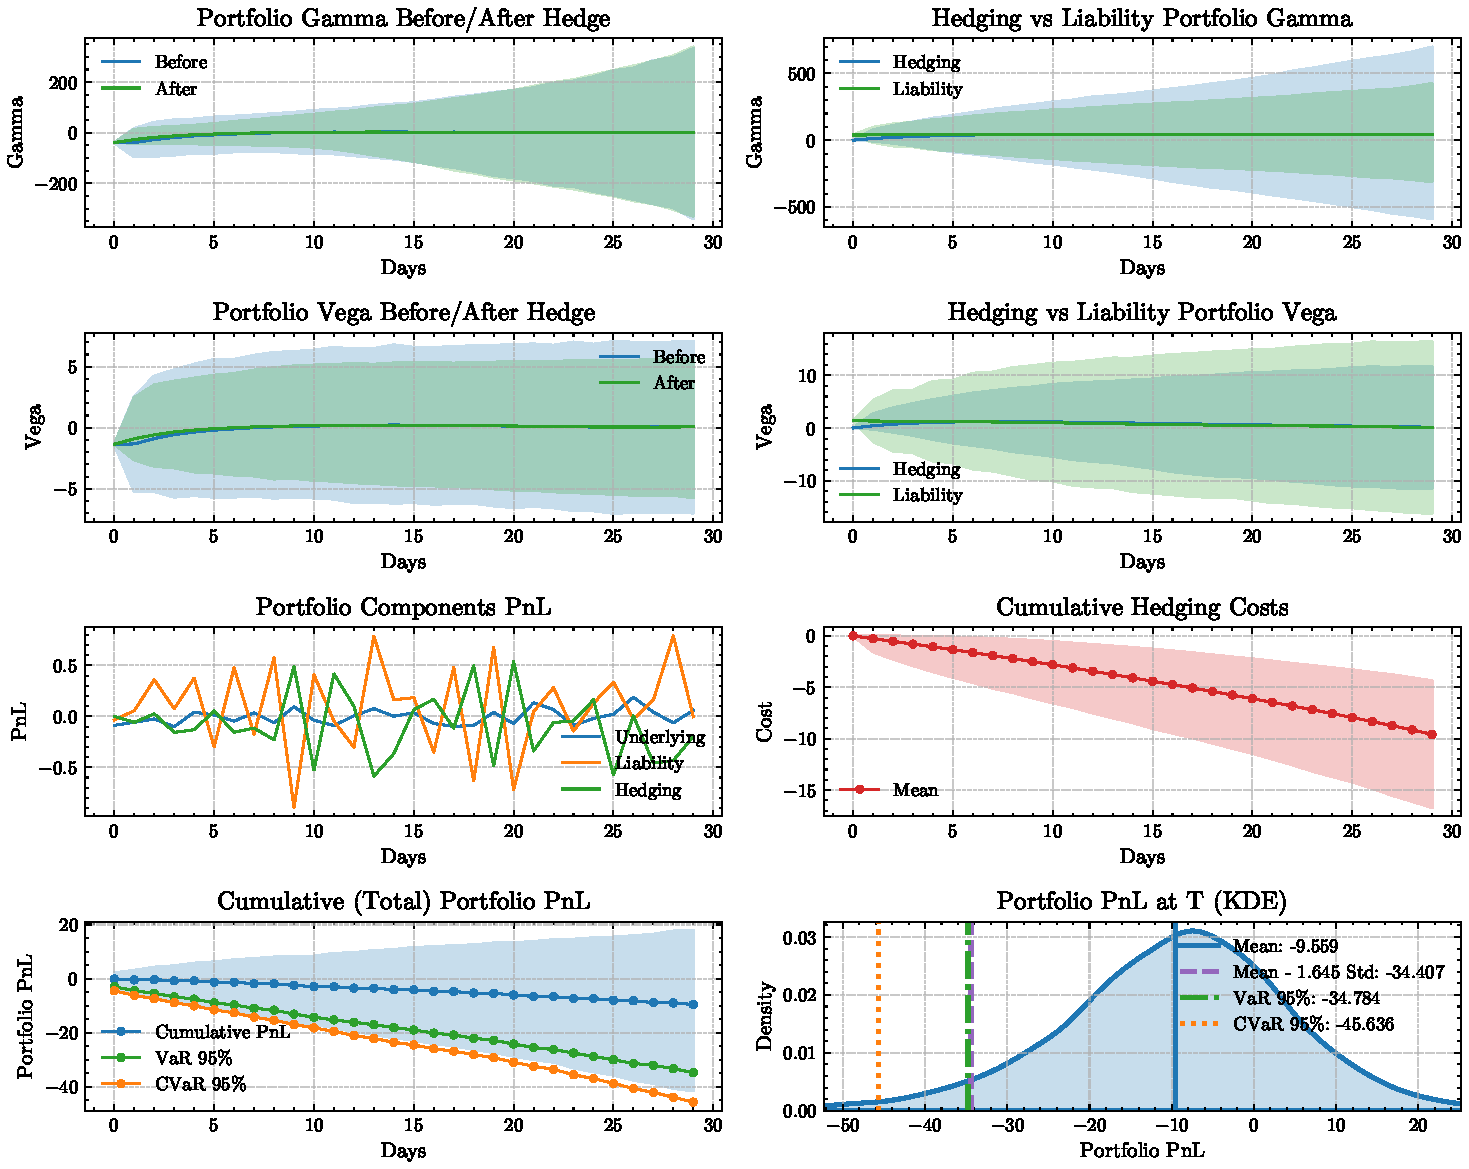
\includegraphics[width=1\linewidth]{figs/Hedging_P_VaR_2.pdf}
    \caption{Visualization of DRL hedging dynamics under the Heston model for a 30-day American put option, optimized for VaR$_{95\%}$ with a 2\% transaction cost under P. The agent responds to sequential option arrivals (60-day maturity) and adjusts a 30-day hedging option accordingly. Subplots (1,1) and (2,1) show the evolution of Gamma and Vega exposures, while (1,2) and (2,2) break these exposures down into liability and hedge components. Subplots (3,1) and (3,2) show average PnL evolution and its relation to transaction cost. Subplot (4,1) relates cost to risk, and (4,2) compares final PnL distributions under different optimization objectives. Shaded areas denote 95\% interquartile ranges over 8,000 episodes.} \label{fig:cvar_viz}
    \vspace{-10pt}
\end{figure*}


\subsubsection{Hedging Dynamics Visualization}
\label{sec:drl_hedging_vis}

\begin{figure*}[t]
    \centering 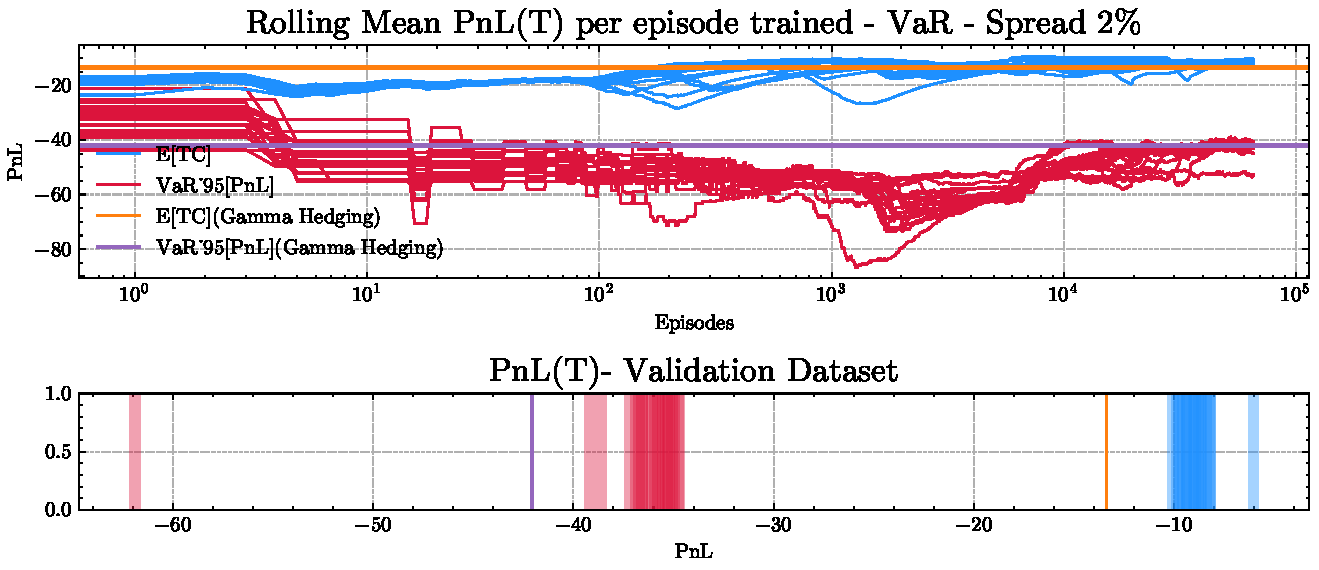
\includegraphics[width=.95\linewidth]{figs/Heston_P_VaR2.pdf}
    \caption{Training and validation performance across 21 independently initialized DRL agents trained under the Heston model using a VaR$_{95\%}$ objective with a 2\% transaction cost. The top panel shows the rolling average PnL and VaR$_{95\%}$ during training; the bottom panel shows the corresponding validation performance over 8000 episodes. Each line represents one agent initialized with a different random seed, trained and evaluated on the same dataset. The wide dispersion in final outcomes highlights the sensitivity of DRL performance to initialization, underscoring the need for multiple training runs and agent selection in high-dimensional hedging problems.}
    \vspace{-15pt}
\label{fig:cvar2}\end{figure*}

The hedging behavior of the DRL agent under the Heston model is visualized in Figure~\ref{fig:cvar_viz}, which depicts results for a 30-day American put option with sequential option arrivals, optimized using a VaR$_{95\%}$ objective and a 2\% transaction cost spread. Subplots (1,1) and (2,1) illustrate how the agent dynamically reduces Gamma and Vega exposures over time, while subplots (1,2) and (2,2) show the respective Greek contributions from each portfolio component (if results for the 0.5\% transaction cost scenario were plotted, they would show more aggressive Gamma and Vega hedging behavior).

Note that the liability portfolio receives randomly arriving options with 60-day time-to-maturity (TTM), whereas the hedging instruments have a fixed 30-day TTM. As a result, the Gamma exposure of the hedge portfolio tends to exceed that of the liabilities, while the opposite holds for Vega. This asymmetry introduces additional complexity into the optimization problem and underscores the flexibility of the DRL agent in adapting its hedging policy to account for non-stationary risk exposures and instrument mismatches.

In addition, subplot (3,1) displays the average PnL of each constituent portfolio, illustrating how the liability and hedge components can exhibit substantial fluctuations that largely offset one another. Subplots (3,2) and (4,1) reveal a near-linear relationship between transaction cost and portfolio risk, indicating that the DRL strategy maintains stable cost-risk trade-offs over the hedging horizon. Subplot (4,2) shows the cumulative PnL distribution at maturity $T$, highlighting how each optimization objective, Mean-Std, VaR, and CVaR, corresponds to a different part of the PnL distribution.

All together, the visualizations provide compelling evidence of the DRL agent’s ability to perform dynamic, cost-aware hedging under stochastic volatility and sequential portfolio construction, adapting effectively to evolving market and risk conditions.

\subsubsection{Training Stability and Agent Selection}
\label{sec:appendix_trainingdynamics}

Figure~\ref{fig:cvar2} shows training and validation results for 21 DRL agents trained under the Heston model with a 2\% transaction cost and VaR$_{95}$ objective. Between agents there is identical architecture, hyperparameters, and training data, with performance variaablity being attributed only to the NNs weights initialization seed. Most agents converge to stable, effective hedging strategies that outperform Delta-Gamma across all risk metrics; with only 1/21 failing to learn an optimal control policy.

The variability in the outcome stems from sensitivity to weight initialization and the inherent stochasticity of policy search and gradient descent in high-dimensional spaces. To reduce uncertainty in the learned policy, we trained multiple agents and selected the best-performing policy based on out of sample results. While most trained agents consistently outperform classical benchmarks, ensuring consistent convergence to the best case, remains a nontrivial challenge. 

In practice, robust policy convergence is as critical as model architecture. Thus, future work may mitigate variability in outcome by employing warm-starts, evolutionary policies, and adaptive scheduling during training.


\section{Experiments under Zero Mean Rate of Return for Equity}\label{sec:experiments-with-zero-drift}

In this section, we conduct a series of controlled experiments where the risk-free rate, equity drift, and equity risk premium are all set to zero, i.e., $r=q=\mu=\lambda_{v}=0\%$. Under these assumptions, the early exercise feature of an American put option lacks economic incentive. Table~\ref{table:hestontable} reports the results under these assumptions, effectively isolating the valuation dynamics from drift and the market price of volatility risk.

This setup enables a focused assessment of the early exercise component’s influence on the performance of the reinforcement learning (RL) algorithm. It also facilitates an indirect comparison with the findings of Cao~\cite{DH_1}, albeit with the use of a different stochastic volatility model (Cao employs SABR with $r = q = \mu = 0\%$) and numerical method used for option evaluations.

In Table \ref{table:hestontable} the RL-based approach continues to outperform rule-based strategies, having slightly worse risk metrics consistently across transaction costs. Additionally, Delta-Vega hedging exhibits the largest relative deterioration in risk, with increases of 7.92\% in VaR95 under 2\% transaction costs relative to Table~\ref{table:hestontableWdrift}. Pure Delta hedging benefits modestly from positive drift, whereas Delta-Gamma hedging shows negligible differences.

Furthermore, the RL strategy under positive drift and negative $\lambda$ exhibits higher vega hedging percentages in Table~\ref{table:hestontableWdrift} versus Table~\ref{table:hestontable}, coresponding to the increased volatility risk which a negative $\lambda$ introduces. Lastly, RL also realizes cost efficiencies, with expected transaction costs reduced by approximately 8–9\% relative to the neutral-drift case. The results of Table~\ref{table:hestontableWdrift} versus Table~\ref{table:hestontable} highlight the robustness of the DRL framework across different drift regimes.

\begin{table*}[t]
\caption{Hedging Results under Heston's stochastic volatility model (with zero drift)}
\begin{adjustbox}{width=1\textwidth}
\begin{tabular}{llccccccc}
\toprule
 & \multicolumn{4}{c}{\textbf{Objective Function Value for}} 
 & \multirow{2}{*}{\shortstack{\textbf{RL Gamma}\\ \textbf{Hedge Ratio}}}
 & \multirow{2}{*}{\shortstack{\textbf{RL Vega}\\ \textbf{Hedge Ratio}}}
 & \multirow{2}{*}{\shortstack{\textbf{Expected RL}\\ \textbf{Transaction Cost}}} \\
\textbf{Objective Function} 
 & \textbf{Delta} 
 & \textbf{Delta-Gamma} 
 & \textbf{Delta-Vega}
 & \textbf{RL} 
 &  &  & \\
\midrule
\multicolumn{8}{l}{\textbf{0.5\% Transaction Cost}} \\
\midrule
Mean-Std & 56.54 & 31.72 & 43.10 & \textbf{\textcolor{darkblue}{26.51}} & 0.43 & 0.26 & 3.81 \\
VaR95    & 55.93 & 31.02 & 41.22 & \textbf{\textcolor{darkblue}{25.57}} & 0.46 & 0.25 & 3.57 \\
CVaR95   & 80.67 & 44.01 & 60.38 & \textbf{\textcolor{darkblue}{35.41}} & 0.45 & 0.26 & 3.72 \\
\midrule
\multicolumn{8}{l}{\textbf{1\% Transaction Cost}} \\
\midrule
Mean-Std & 56.54 & 35.15 & 49.51 & \textbf{\textcolor{darkblue}{29.55}} & 0.32 & 0.19 & 5.76 \\
VaR95    & 55.93 & 34.72 & 47.96 & \textbf{\textcolor{darkblue}{29.00}} & 0.36 & 0.20 & 5.87 \\
CVaR95   & 80.67 & 47.74 & 67.45 & \textbf{\textcolor{darkblue}{40.36}} & 0.38 & 0.17 & 5.91 \\
\midrule
\multicolumn{8}{l}{\textbf{2\% Transaction Cost}} \\
\midrule
Mean-Std\ & 56.54 & 42.15 & 62.66 & \textbf{\textcolor{darkblue}{34.77}} & 0.29 & 0.18 & 9.88 \\
VaR95    & 55.93 & 42.09 & 61.98 & \textbf{\textcolor{darkblue}{34.84}} & 0.23 & 0.16 & 8.78 \\
CVaR95\footnotemark[3]   & 80.67 & 55.32 & 81.83 & \textbf{\textcolor{darkblue}{45.43}} & 0.23 & 0.16 & 8.78 \\
\bottomrule
\end{tabular}
\end{adjustbox}
\justifying \small
Comparison of hedging strategies under stochastic volatility using the Heston model. Risk and cost outcomes are reported for classical Delta, Delta-Gamma, Delta-Vega, and DRL-based hedging across three transaction cost levels (0.5\%, 1\%, 2\%). DRL policies are trained using the D4PG-QR algorithm with Mean-Std, VaR$_{95\%}$ or CVaR$_{95\%}$ objectives. For each strategy and objective, we report the corresponding loss metric value. The final three columns summarize the DRL agent’s average Gamma hedge ratio, Vega hedge ratio, and expected transaction cost over 8,000 evaluation paths. Gamma/Vega hedge ratios denote the average proportion of risk neutralized across the hedging horizon. The expected transaction costs for Delta-Gamma are 3.35, 6.69, and 13.39 for the respective transaction cost regimes; for Delta-Vega, the values are 6.23, 12.45, and 24.92. Delta hedging is assumed to be frictionless, thus risk values remain constant through different transaction costs regimes.
\vspace{-5pt}
\label{table:hestontable}
\end{table*}


\paragraph*{Choosing an Objective Function.}
In this section, we train DRL agents with all three objective functions. Based on those results, Table ~\ref{tab:1pct_agents} bellow reveals that the choice of objective function does not significantly impact the risk metrics which the agent was not directly optimized for. Thus, in our experiments agents trained to minimize VaR95 also achieved strong performance in terms of CVaR95 and Mean-Std, and vice versa. This observation is consistent with Figure~\ref{fig:cvar_viz}, subplot (4,2), which shows that all three optimization objectives effectively targeting neighboring regions in the resulting PnL distribution (specially in the case of Mean-Std and VaR95). Consequently, to reduce training costs in the more demanding stochastic volatility setting with early-exercise features, we restricted training to the VaR95 objective and only report those results in Table~\ref{table:hestontableWdrift}.

\begin{table}[width=\linewidth,cols=5,pos=H]
  \centering
  \caption{Performance of 1\%-transaction costs-trained agents across risk metrics}
  \label{tab:1pct_agents}
  \begin{tabular}{@{}lcccc@{}}
    \toprule
    \textbf{Objective F.} 
      & \textbf{Mean–Std} 
      & \textbf{VaR$_{95\%}$} 
      & \textbf{CVaR$_{95\%}$} 
      & $\mathbb{E}[\text{TC}]$ \\
    \midrule
    Mean–Std 
      & $29.55$ 
      & $29.17$ 
      & $39.92$ 
      & $5.76$ \\
    VaR95
      & $29.27$ 
      & $29.00$ 
      & $38.92$ 
      & $5.87$ \\
    CVaR95
      & $30.07$ 
      & $29.74$ 
      & $40.36$ 
      & $6.16$ \\
    \bottomrule
  \end{tabular}
\end{table}

These results suggest that the DRL policy exhibits robustness across different risk metrics, even when trained with respect to only one. Nevertheless, VaR emerges as a particularly practical objective. It is less sensitive to extreme outliers during training than CVaR. Which could explain why VaR optimized agent outperforms the CVaR optimized agent in the CVaR metric in Table ~\ref{tab:1pct_agents}. Additionally, the VaR objective function corresponds to a fixed quantile of the PnL distribution, offering a more stable and interpretable target compared to the Mean-Std objective.

\footnotetext[2]{CVaR95 and Mean-Std Metrics are reported based on the performance of an agent optimized with the VaR95 objective function.}


\subsection{Comparison to Cao's \cite{DH_1} Results} \label{sec:cao_comparison}

\begin{table*}[pos=t]
\caption{Our Results compared to Cao's \cite{DH_1} results}
\begin{adjustbox}{width=1\textwidth}
\begin{tabular}{lcccccc}
\toprule
 & \multicolumn{3}{c}{\textbf{Our Results (Heston, Amer. Put)}} 
 & \multicolumn{3}{c}{\textbf{Cao's Results (SABR, Euro. Call)}} \\
\cmidrule(lr){2-4} \cmidrule(lr){5-7}
\textbf{Objective Function} 
 & \textbf{Delta-Gamma Value} 
 & \textbf{RL Value} 
 & \textbf{\% Reduction} 
 & \textbf{Delta-Gamma Value} 
 & \textbf{RL Value} 
 & \textbf{\% Reduction} \\
\midrule
\multicolumn{7}{l}{\textbf{0.5\% Transaction Cost}} \\
\midrule
Mean-Std & 31.72 & 26.51 & \textbf{16.43\%} & 19.46 & 17.76 & \textbf{8.74\%} \\
VaR95    & 31.02 & 25.57 & \textbf{17.57\%} & 19.23 & 19.31 & \textbf{-0.42\%} \\
CVaR95   & 44.01 & 35.41 & \textbf{19.54\%} & 27.53 & 26.06 & \textbf{5.34\%} \\
\midrule
\multicolumn{7}{l}{\textbf{1\% Transaction Cost}} \\
\midrule
Mean-Std & 35.15 & 29.55 & \textbf{15.93\%} & 23.06 & 20.03 & \textbf{13.13\%} \\
VaR95    & 34.72 & 29.00 & \textbf{16.48\%} & 23.02 & 20.22 & \textbf{12.16\%} \\
CVaR95   & 47.74 & 40.36 & \textbf{15.46\%} & 31.55 & 26.81 & \textbf{15.03\%} \\
\midrule
\multicolumn{7}{l}{\textbf{2\% Transaction Cost}} \\
\midrule
Mean-Std & 42.15 & 34.77 & \textbf{17.51\%} & 30.51 & 24.17 & \textbf{20.77\%} \\
VaR95    & 42.09 & 34.84 & \textbf{17.24\%} & 30.67 & 23.85 & \textbf{22.23\%} \\
CVaR95\footnotemark[3]   & 55.32 & 45.43 & \textbf{17.88\%} & 39.79 & 31.57 & \textbf{20.67\%} \\
\bottomrule
\end{tabular}
\end{adjustbox}
\justifying \small
Comparison of DRL hedging results for American puts under the Heston model (our work) versus European calls under the SABR model as presented by Cao~\cite{DH_1}. The percentage reduction is computed as $\bigl(\text{Delta-Gamma} - \text{RL}\bigr)/\text{Delta-Gamma} \times 100\%$, and reflects the improvement in the objective function value achieved by the DRL policy relative to the Delta-Gamma baseline.
\label{tab:resultsComparisonWithCao}
\end{table*}


Table~\ref{tab:resultsComparisonWithCao} compares our DRL hedging results for American put options under Heston dynamics with zero drift and market price vol-premium, with those reported by Cao~\cite{DH_1}, who studied European call options under the SABR model and also zero drift and zero market price vol-premium. Despite differences in option type, stochastic model, and hedging setup, the relative improvements achieved by the DRL agent are comparable in magnitude across many objective functions and transaction cost levels. With the biggest difference being that our method achieves consistent reductions in risk across all objectives and transaction costs, where in Cao's case the RL's risk reduction increase with transaction costs. This could be attributed to the different stochastic model of choice or/and the option valuation methodology.


\section{Robustness to Model Misspecification}
\label{sec:robustness}

\begin{table}[width=\linewidth,cols=4,pos=h]
\caption{Robustness testing over different bumped parameters}
\label{tbl:robustness}
\begin{tabular*}{\tblwidth}{@{} LLLL@{} }
\toprule
Parameter & CVaR\textsubscript{95} & transaction costs & Observations \\
\midrule
\multicolumn{4}{l}{\em Initial Volatility ($v_0$)} \\
\midrule
$v_0=0.1$ & 29.92 & 6.24 & Reduced risk, reduced cost. \\
$v_0=0.2$ & 39.79 & 9.01 & Reduced risk, reduced cost. \\
$v_0=0.3$ & 45.15 & 9.37 & -- \\
$v_0=0.4$ & 60.09 & 16.28 & Larger risk, larger cost. \\
$v_0=0.5$ & 72.44 & 24.84 & Larger risk, larger cost. \\
\midrule
\multicolumn{4}{l}{\em Volatility-of-Volatility ($\xi$)} \\
\midrule
$\xi=0.1$ & 33.65 & 9.75 & Reduced risk, larger cost. \\
$\xi=0.2$ & 40.12 & 9.51 & Reduced risk, similar cost. \\
$\xi=0.3$ & 45.15 & 9.37 & -- \\
$\xi=0.4$ & 59.15 & 9.38 & Larger risk, similar cost. \\
$\xi=0.5$ & 68.98 & 9.46 & Larger risk, similar cost. \\
\midrule
\multicolumn{4}{l}{\em Mean Reversion Speed ($\kappa_{\mathbb{P}}$)} \\
\midrule
$\kappa_{\mathbb{P}}=0.5$ & 51.71 & 9.38 & Larger risk, similar cost. \\
$\kappa_{\mathbb{P}}=0.8$ & 50.18 & 9.38 & Larger risk, similar cost. \\
$\kappa_{\mathbb{P}}=1.0$ & 45.15 & 9.37 & -- \\
$\kappa_{\mathbb{P}}=1.2$ & 48.35 & 9.38 & Larger risk, similar cost. \\
$\kappa_{\mathbb{P}}=1.5$ & 47.05 & 9.38 & Larger risk, similar cost. \\
\midrule
\multicolumn{4}{l}{\em Correlation ($\rho$)} \\
\midrule
$\rho=-0.9$ & 47.65 & 9.03 & Larger risk, reduced cost. \\
$\rho=-0.8$ & 48.48 & 9.21 & Larger risk, similar cost. \\
$\rho=-0.7$ & 45.15 & 9.37 & -- \\
$\rho=-0.6$ & 49.72 & 9.54 & Larger risk, similar cost. \\
$\rho=-0.5$ & 50.16 & 9.68 & Larger risk, similar cost. \\
\midrule
\multicolumn{4}{l}{\em Long Term Variance ($\theta_{\mathbb{P}}$)} \\
\midrule
$\theta_{\mathbb{P}}=0.03$ & 49.49 & 9.31 & Larger risk, similar cost. \\
$\theta_{\mathbb{P}}=0.06$ & 49.34 & 9.35 & Larger risk, similar cost. \\
$\theta_{\mathbb{P}}=0.09$ & 45.15 & 9.37 & -- \\
$\theta_{\mathbb{P}}=0.12$ & 49.18 & 9.43 & Larger risk, similar cost. \\
$\theta_{\mathbb{P}}=0.15$ & 49.17 & 9.51 & Larger risk, similar cost. \\
\bottomrule
\end{tabular*}

\justifying \small
Robustness evaluation of DRL hedging performance under Heston model parameter misspecification. Each row shows the resulting CVaR$_{95\%}$ and expected transaction cost (transaction costs) when a single parameter is perturbed from its baseline value: $\{v_0=0.3,\ \xi=0.3,\ \kappa_{\mathbb{P}}=1.0,\ \rho=-0.7,\ \theta_{\mathbb{P}}=0.09\}$. The third column provides qualitative observations. Results are averaged over 8,000 episodes using the same DRL policy trained under baseline parameters with a 2\% transaction cost and CVaR$_{95\%}$ objective. The 95\% confidence intervals for baseline CVaR$_{95\%}$ and transaction costs are 1.59 and 0.36, respectively.
\vspace{-5pt}
\end{table}

In real-world applications, Heston model parameters are rarely calibrated with perfect accuracy, resulting in discrepancies between the assumed model dynamics and the true behavior of the market. This section evaluates the robustness of the deep reinforcement learning hedging policy under such parameter mismatches. Where the realized market conditions (parameters) vary from the initial assumed (calibrated) ones. For these experiments we assumed $r=\mu=q=\lambda_{v}=0$ and parameters $\kappa_{\mathbb{P}}, \theta_{\mathbb{P}}, \xi, \rho$ are assumed to be constant for the duration of the simulation. 

Robustness is a critical requirement for practical deployment, as it ensures that the learned policy maintains effective risk mitigation even when model assumptions are violated. A robust strategy should generalize well to moderate shifts in key parameters, avoiding catastrophic performance degradation due to calibration errors or regime shifts in volatility dynamics.

As shown in Table~\ref{tbl:robustness} and Figure~\ref{fig:enter-label} in general small shifts in Heston parameters lead to small differences in the value of CVaR\textsubscript{95} indicating that the DRL hedging strategy generally maintains its expected risk metrics and transaction costs. This robustness is particularly evident for perturbations in the parameters $\{\theta_{\mathbb{P}}, \rho, \kappa_{\mathbb{P}}\}$, where the impact on risk and cost remains modest. In contrast, shifts in $\{v_0, \xi\}$ lead to more pronounced changes in both the risk and cost profiles, indicating greater sensitivity to initial variance $v_0$ and volatility-of-volatility $\xi$.

\footnotetext[3]{The CVaR$_{95}$ metric is from the VaR$_{95}$-optimized agent, which outperforms the CVaR$_{95}$-optimized agent on its own metric, as shown in Table~\ref{tab:1pct_agents}.}

Most notably, initial variance $v_0$ exhibits a monotonic relationship with cost: higher than expected $v_0$ increases both expected costs and tail risk, and lower than expected $v_0$ results to lower costs and tail risk. One potential approach would be to use variance swaps or volatility futures to reduce the sensitivity to changes in realized volatility. Table~\ref{tbl:robustness} showcases the significance of correctly estimating $v_0$ and $\xi$ at the time of hedge initiation. 

\begin{figure}[pos=t]
    \centering
    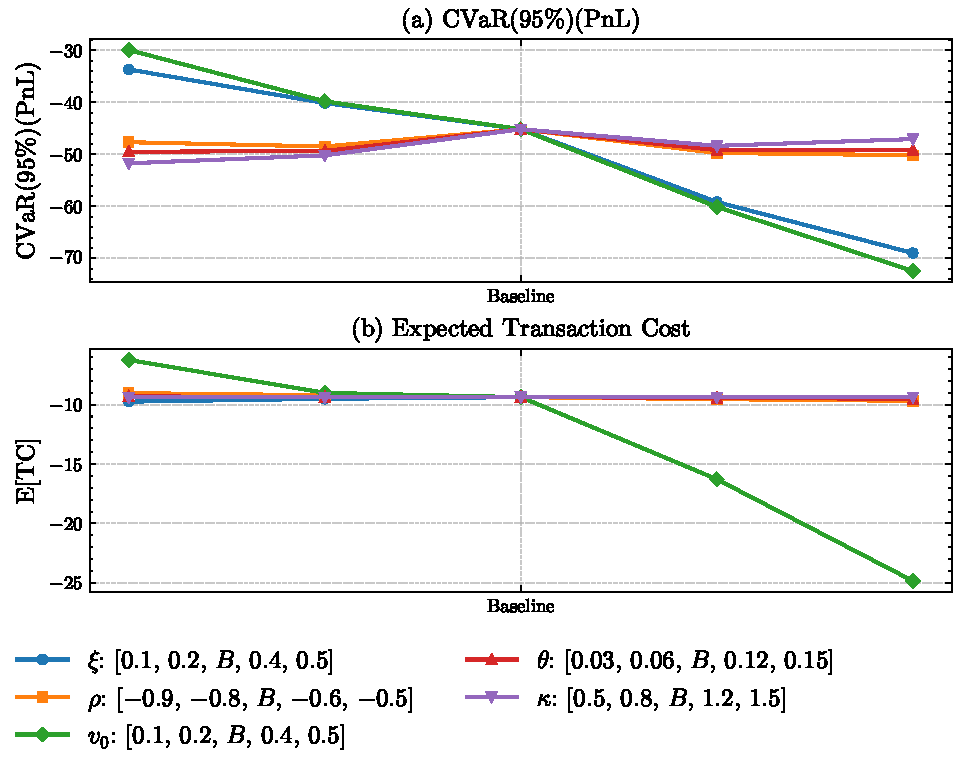
\includegraphics[width=1\linewidth]{figs/parameter_sensitivity.pdf}
    \vspace{-10pt}
    \caption{Robustness Testing on Heston model: Out of sample evaluation of the CVaR$_{95\%}$, (2\% transaction costs) trained agent on bumped parameter values}
    \label{fig:enter-label}
    \vspace{-15pt}
\end{figure}


\section{Conclusion}
\label{sec:conclusion}

We proposed a deep reinforcement learning based hedging framework for managing Gamma and Vega exposure in American put options under stochastic volatility. The approach combines the Quadratic-Exponential scheme for accurate simulation of Heston paths with the Modified Craig–Sneyd finite difference scheme for precise valuation of American options, and a cutting-edge DRL framework (D4PG-QR) for option hedging. To the best of our knowledge, this is the first study to address higher-order hedging of American options within the Heston framework using DRL.

Our results demonstrate that the DRL-based strategy consistently achieves lower risk and transaction costs compared to fully hedged Gamma/Vega strategies. By selectively hedging higher-order exposures, the agent dynamically optimizes the trade-off between tail-risk reduction and cost efficiency.

We further assess the method's robustness to parameter misspecification and observe that the learned policy demonstrates stable performance, reinforcing its practical viability in realistic market conditions with imperfect calibration. Additionally, under the physical measure $\mathbb{P}$ and a positive risk-free rate, which incentivizes optimal early exercise for American options in specific scenarios, the RL agent achieves a slightly lower risk profile at equivalent or lower hedging costs. This suggests that the RL agent offers robust risk and cost reduction across different drift regimes for the underlying and the risk-free-rate.

An analysis of the training process in Section~\ref{sec:appendix_trainingdynamics} reveals sensitivity to the NNs weights initialization, highlighting the need for subsequent work on ensuring robust optimization with a single agent, but with the current setup, multiple training runs are required to select the best-performing agent.

Finally, we provide a comparison with the work of Cao~\cite{DH_1}. Despite differences in modeling assumptions, we observe a somewhat comparable relative reduction in risk, reinforcing the effectiveness of a DRL (D4PG-QR) hedging approach.

\section{Future Research Directions}
\label{sec:FutureDirections}

While our results demonstrate the effectiveness of DRL for higher-order hedging under stochastic volatility, several extensions remain open for exploration.

First, instead of starting with a single option, future work could start from a given portfolio of options, e.g. calls, puts, European, American, swaps and futures across various strikes and maturities. This would better reflect real-world trading environments and increase policy applicability.

Second, expanding the action space to include additional hedging instruments, such as variance swaps or options with different maturities and strikes, could enhance the agent’s ability to control complex sensitivities, including higher-order Greeks.

Third, more realistic modeling of transaction costs; varying by strike, maturity, and market conditions; would increase exactness. Similarly, simulating the arrival of new liabilities using historical trade data would align training environments more closely with institutional settings.

Fourth, incorporating jump-diffusion models would allow the framework to better capture short-term price shocks and improve hedging accuracy for short-dated options. Additionally, modeling parameter uncertainty during training (e.g., randomizing Heston parameters) could improve robustness to market regime changes.

From a computational perspective, improvements in PDE interpolation schemes could significantly reduce evaluation overhead. This includes employing Chebyshev interpolation or structured nearest-neighbor grids to accelerate price and Greek lookups without compromising accuracy.


Lastly, algorithmic performance could benefit from more tuned DRL architectures. Enhancements might include integrating additional higher-order Greeks into the state space (Charm $\big( \frac{\partial \Delta}{\partial t} \big)$, Veta $\big( \frac{\partial \mathcal{V}}{\partial t} \big)$, Color $\big( \frac{\partial \Gamma}{\partial t} \big)$), employing scheduling techniques for learning rate decay, or using better initialization strategies for the NNs in the actor-critic NNs. Such enhancements are more geared to increase the quality and the speed of training DRL agents.

\subsection*{Code and Data Availability}
This study relies exclusively on simulated data. The source code and scripts 
used to generate the results are publicly available under 
\href{https://github.com/ithakis/DRL-Hedging-AmericanOptions}{github.com/ithakis/DRL-Hedging-AmericanOptions}.

% References
\bibliographystyle{cas-model2-names}
\bibliography{Bibliography.bib}


% \appendix


\end{document}
